\section{Background}
Evolutionary Algorithms have been used to develop similar solutions before. Examples of previous  applications are tables[See figure \ref{fig:hornby_tables}] where the optimisation parameters were height of the support structure, stability of the structure and maximization of surface area.
\begin{figure}[ht]
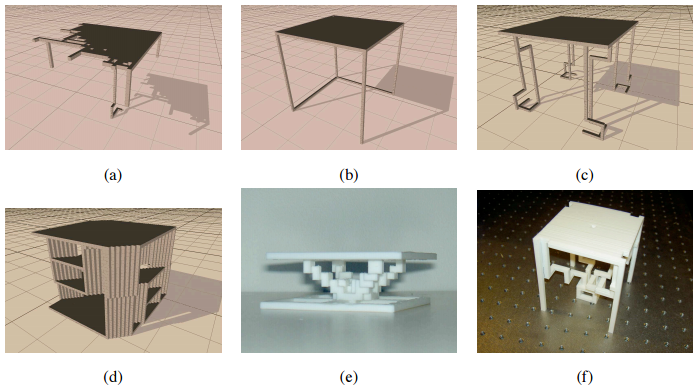
\includegraphics[scale=.6]{content/img/tables}
\label{fig:hornby_tables}\\
\caption{Image of Hornsby tables\cite{paper:ev4} }
\end{figure}

While the evolution of tables has some similarities to seating they are inherent different in the sense that maximized surface area might not be ideal for a chair nor would very high legs be seing the physical attributes of humans usually constrain us to some specific height range which is optimal for the average persons seating comfort.
